\scanpage{5}
once again that it is only the \uline{germ}
of the $\varphi_\xi$ that is defined
(modulo restriction to a subgroup of finite
index). [If $X$ maps injectively
into an extension of an abelian variety by a
torus, then $\xi$ is known when one
knows this germ
\[
(11)\qquad\varphi_\xi\in\underset{\substack{\Gamma'\subset\Gamma\\\text{open}}}{\lim\limits_{\longrightarrow}}
\operatorname{Hom}(\Gamma',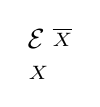
\begin{tikzpicture}[baseline=(ext.base)]
\node[inner sep=0pt] (ext) at (0,0) {$\mathcal E$};
\node[anchor=base west,inner sep=0pt,font=\scriptsize] at (.20,-.10)
 {$\deleted{\unsure{\overline X}}$};
\node[inner sep=0pt,font=\scriptsize] at (.03,-.43) {$\inserted{X}$};
\end{tikzpicture})
/\operatorname{Int}(\pi_1(X),\mathcal E_X)
\]
[and $=$ the image of $\varphi_\xi$ in a suitable abelian
$H^1$\ldots] ]

\textcircled{4}
\[
(12)\qquad\text{Let }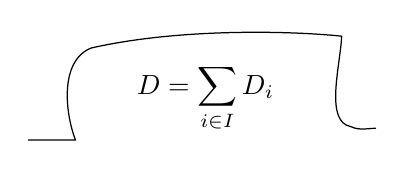
\begin{tikzpicture}[baseline=(div.base),line cap=round,line join=round]
\node[inner sep=0pt] (div) at (2.15,0) {$\displaystyle D=\sum_{i\in I}D_i$};
% Open underneath: left outward foot, rounded roof, curled right foot.
\draw[line width=.45pt] (-.10,-.53)--(.50,-.53)
 ..controls(.37,-.20)and(.29,.48)..(.70,.64)
 ..controls(1.80,.89)and(3.20,.86)..(3.88,.79)
 ..controls(3.86,.40)and(3.66,-.30)..(4.00,-.36)
 ..controls(4.10,-.41)and(4.22,-.38)..(4.31,-.38);
\end{tikzpicture}\quad\text{be a divisor }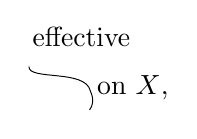
\begin{tikzpicture}[baseline=(sur.base)]
\node[anchor=base west,inner sep=0pt] (sur) at (.48,0) {on $X$,};
\node[anchor=base west,inner sep=0pt] at (-.34,.60) {\inserted{effective}};
\draw[line width=.35pt] (-.38,.35)..controls(-.39,.17)and(.34,.32)..(.40,.04)
 ..controls(.45,-.07)and(.43,-.15)..(.39,-.20);
\end{tikzpicture}
\]
($I$ the set of its irreducible components) without multiple components,
suppose that $X$ is regular 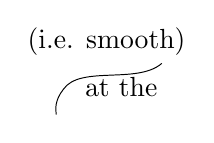
\begin{tikzpicture}[baseline=(enles.base)]
\node[anchor=base west,inner sep=0pt] (enles) at (.63,0) {at the};
\node[anchor=base west,inner sep=0pt] at (-.10,.61) {\inserted{(i.e. smooth)}};
\draw[line width=.35pt] (1.61,.42)..controls(1.30,.15)and(.57,.40)..(.36,.09)
 ..controls(.25,-.05)and(.26,-.16)..(.27,-.23);
\end{tikzpicture}
generic points of each $D_i$. Let \deleted{$X_I$}
\[
(13)\qquad X'=X-\operatorname{supp}D
\]
and consider the subgroup $\mathcal G_{\unsure{X',X|X;X}}$ of
$\mathcal G_X$ which leaves $D$ invariant. We shall denote it by 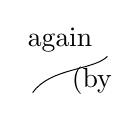
\begin{tikzpicture}[baseline=(par.base)]
\node[anchor=base west,inner sep=0pt] (par) at (.61,0) {(by};
\node[anchor=base west,inner sep=0pt] at (.05,.53) {\inserted{again}};
\draw[line width=.35pt] (1.07,.40)..controls(.89,.22)and(.35,.26)..(.12,-.06);
\end{tikzpicture}
abuse of notation) $\mathcal G_{X'}$, 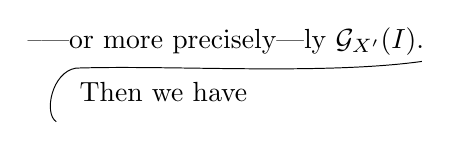
\begin{tikzpicture}[baseline=(alors.base)]
\node[anchor=base west,inner sep=0pt] (alors) at (.47,0) {Then we have};
\node[anchor=base west,inner sep=0pt] (refinement) at (-.19,.67)
 {\inserted{\unsure{--|or} more precise\unsure{ly|ly} $\mathcal G_{X'}(I)$.}};
\draw[line width=.35pt] ([xshift=-1pt,yshift=-2pt]refinement.south east)
 ..controls(3.55,.33)and(1.65,.46)..(.43,.42)
 ..controls(.12,.37)and(.02,-.16)..(.18,-.26);
\end{tikzpicture}
\mspage{4}
